\begin{minipage}[h!]{0.5\textwidth}
  \centering
  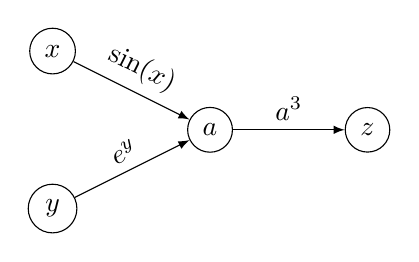
\begin{tikzpicture}[>=latex]

    \path (0,1) node [circle,draw](var_x){$x$};
    \path (0,-1) node [circle,draw](var_y){$y$};
    \path (2,0) node [circle,draw](var_a){$a$};
    \path (4,0) node [circle,draw](var_z){$z$};
    % \path[red] (0,1.5) node(x1){$x_1$} (0,0) node(x2){$x_2$} (0,-1.5) node(x3){$x_3$};
    \draw[->] (var_x) -- node[above,sloped]{$\sin(x)$} (var_a);
    \draw[->] (var_y) -- node[above,sloped]{$e^y$} (var_a);
    \draw[->] (var_a) -- node[above,sloped]{$a^3$} (var_z);

  \end{tikzpicture}

\end{minipage}
\begin{minipage}[h!]{0.5\textwidth}
  \begin{align*} % or align*
    a(x,y) &= \sin(x) + e^y \\
    z(a(x,y)) &= a^3(x,y) = \left(\sin(x) + e^y\right)^3 \\[3ex]
    \partderiv{z}{x} &= \partderiv{a}{x} \cdot  \partderiv{z}{a} = \cos(x) \cdot 3a^2 \\[0.5ex]
    \partderiv{z}{y} &= \partderiv{a}{y} \cdot \partderiv{z}{a} = e^y \cdot 3a^2
  \end{align*}
\end{minipage}
%%% Local Variables:
%%% mode: latex
%%% TeX-master: "../figs"
%%% End:
